\chapter{Experiments and Applications}\label{chap:4}
In this chapter describe the two main experiments we built to collect data and analyze our system. Ten people were involved in the data collection. Each experiment will be presented in terms of goals, procedures and results. Moreover, we will show a couple of applications for the system involving also a ground robot. Those applications are not only discussed, but also demonstrated with a kobuki, allowing us to draw qualitative results.
\section{Pointing Feedback Experiment}
\subsection{Setup}
\begin{figure}
	\centering
	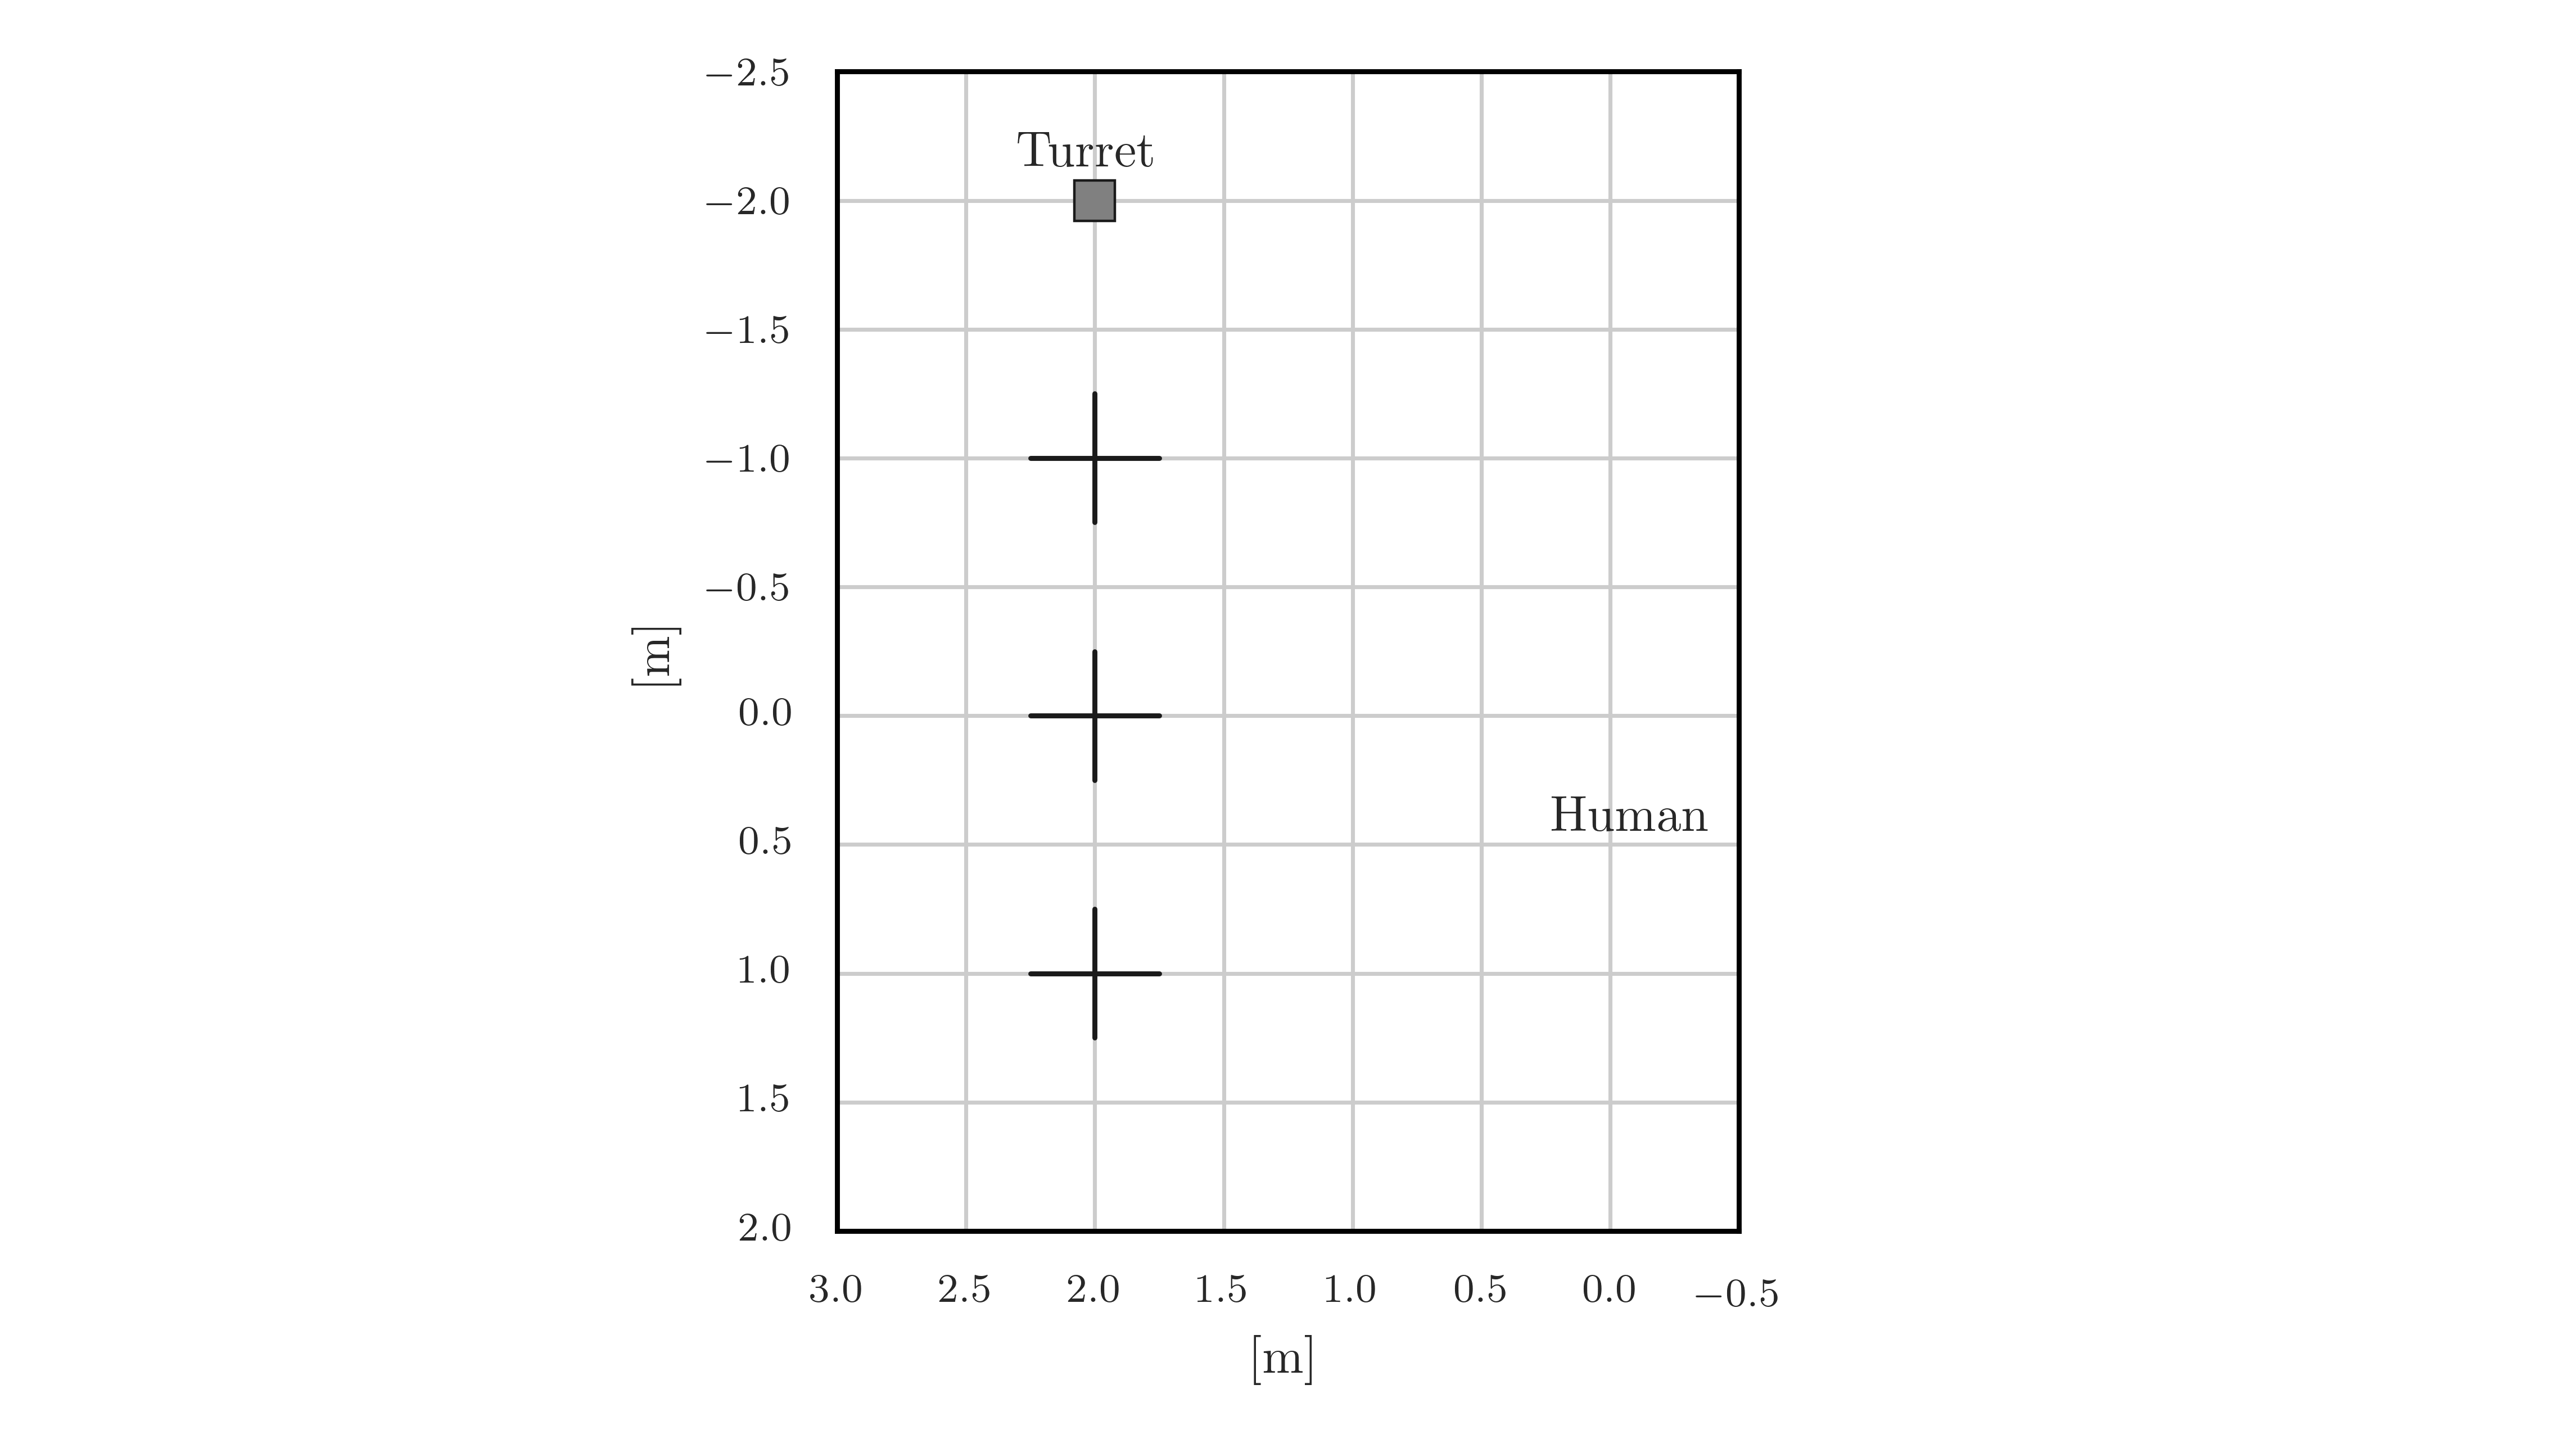
\includegraphics[width=\textwidth]{img/pointingExpSetup.png}%
	\caption{Pointing Experiment Setup (Black Crosses Are Ground Targets)}
	\label{fig:pointingExpSetup}
\end{figure}
We place the turret and three ground targets in known positions. The user is placed in front of the second target, oriented perpendicularly to the line connecting the targets. Figure \ref{fig:pointingExpSetup} shows that setup. The relative localization between the human and the turret is known a priori, so we are not performing any relloc. The user is wearing the IMU and we are collecting his pointing data.\\
The user has to point each target first without any additional visual feedback, so he has to rely solely on his perception. Second, he has to point again with the visual feedback provided by the laser dot. Those are the steps composing each iteration of the experiment (one for each target):
\begin{itemize}
    \item after a countdown, the user points the target without feedback;
    \item the user keeps pointing for 5 seconds;
    \item after a sound feedback, the user can rest his arm;
    \item after a countdown, the user points the target with the laser; feedback;
    \item the user keeps pointing for 5 seconds;
    \item after a sound feedback, the user can rest his arm.
\end{itemize}
Each user has to perform that loop three time for each target, for a total of nine iterations.
\subsection{Goals}
The performance of the interface crucially relies on operator’s perception. Due to simplifications in the pointing model that we use and various sensory errors, the estimated frame transformations and the pointing are expected to be imprecise.\\
With that experiment we want to understand if availability of visual feedback is useful and thus improves the pointing accuracy. This is why we ask users to drive the laser dot to the target, where the laser dot represents the location where the system thinks the user is pointing. Comparing results with and without feedback, we can understand if providing that feedback helps users to timely adapt to any misalignments.

\subsection{Results}
First, we can look at the users' trajectories with and without feedback in figure \ref{fig:userTrajectories}. We can immediately see that without feedback users go straight to their goal point, but that point, for the system, does not correspond to the target. With feedback, on the contrary, users are able to tell the system to point at the target. This intuition can be see in figure \ref{fig:distanceComparison} and is further confirmed by figure \ref{fig:avgDistance}: without feedback, users quickly reach an average distance from the target of 0.5 m but do not improve any further. When the feedback is provided, distance decreases to almost 0 within 5 seconds. This is expected as the system has intrinsic inaccuracies (for example in the reconstruction of pointing rays) which the user is unable to see and correct. 

This demonstrates that real-time feedback is a key component for our system. This justifies all the work done to build the turret, as, while with fast moving robots (e.g. a drone), the robot position itself can be the feedback, for slow moving machine (e.g. a ground robot) the laser dot represents a valid possibility, as also our demos with the kobuki show.

\begin{figure}
	\centering
	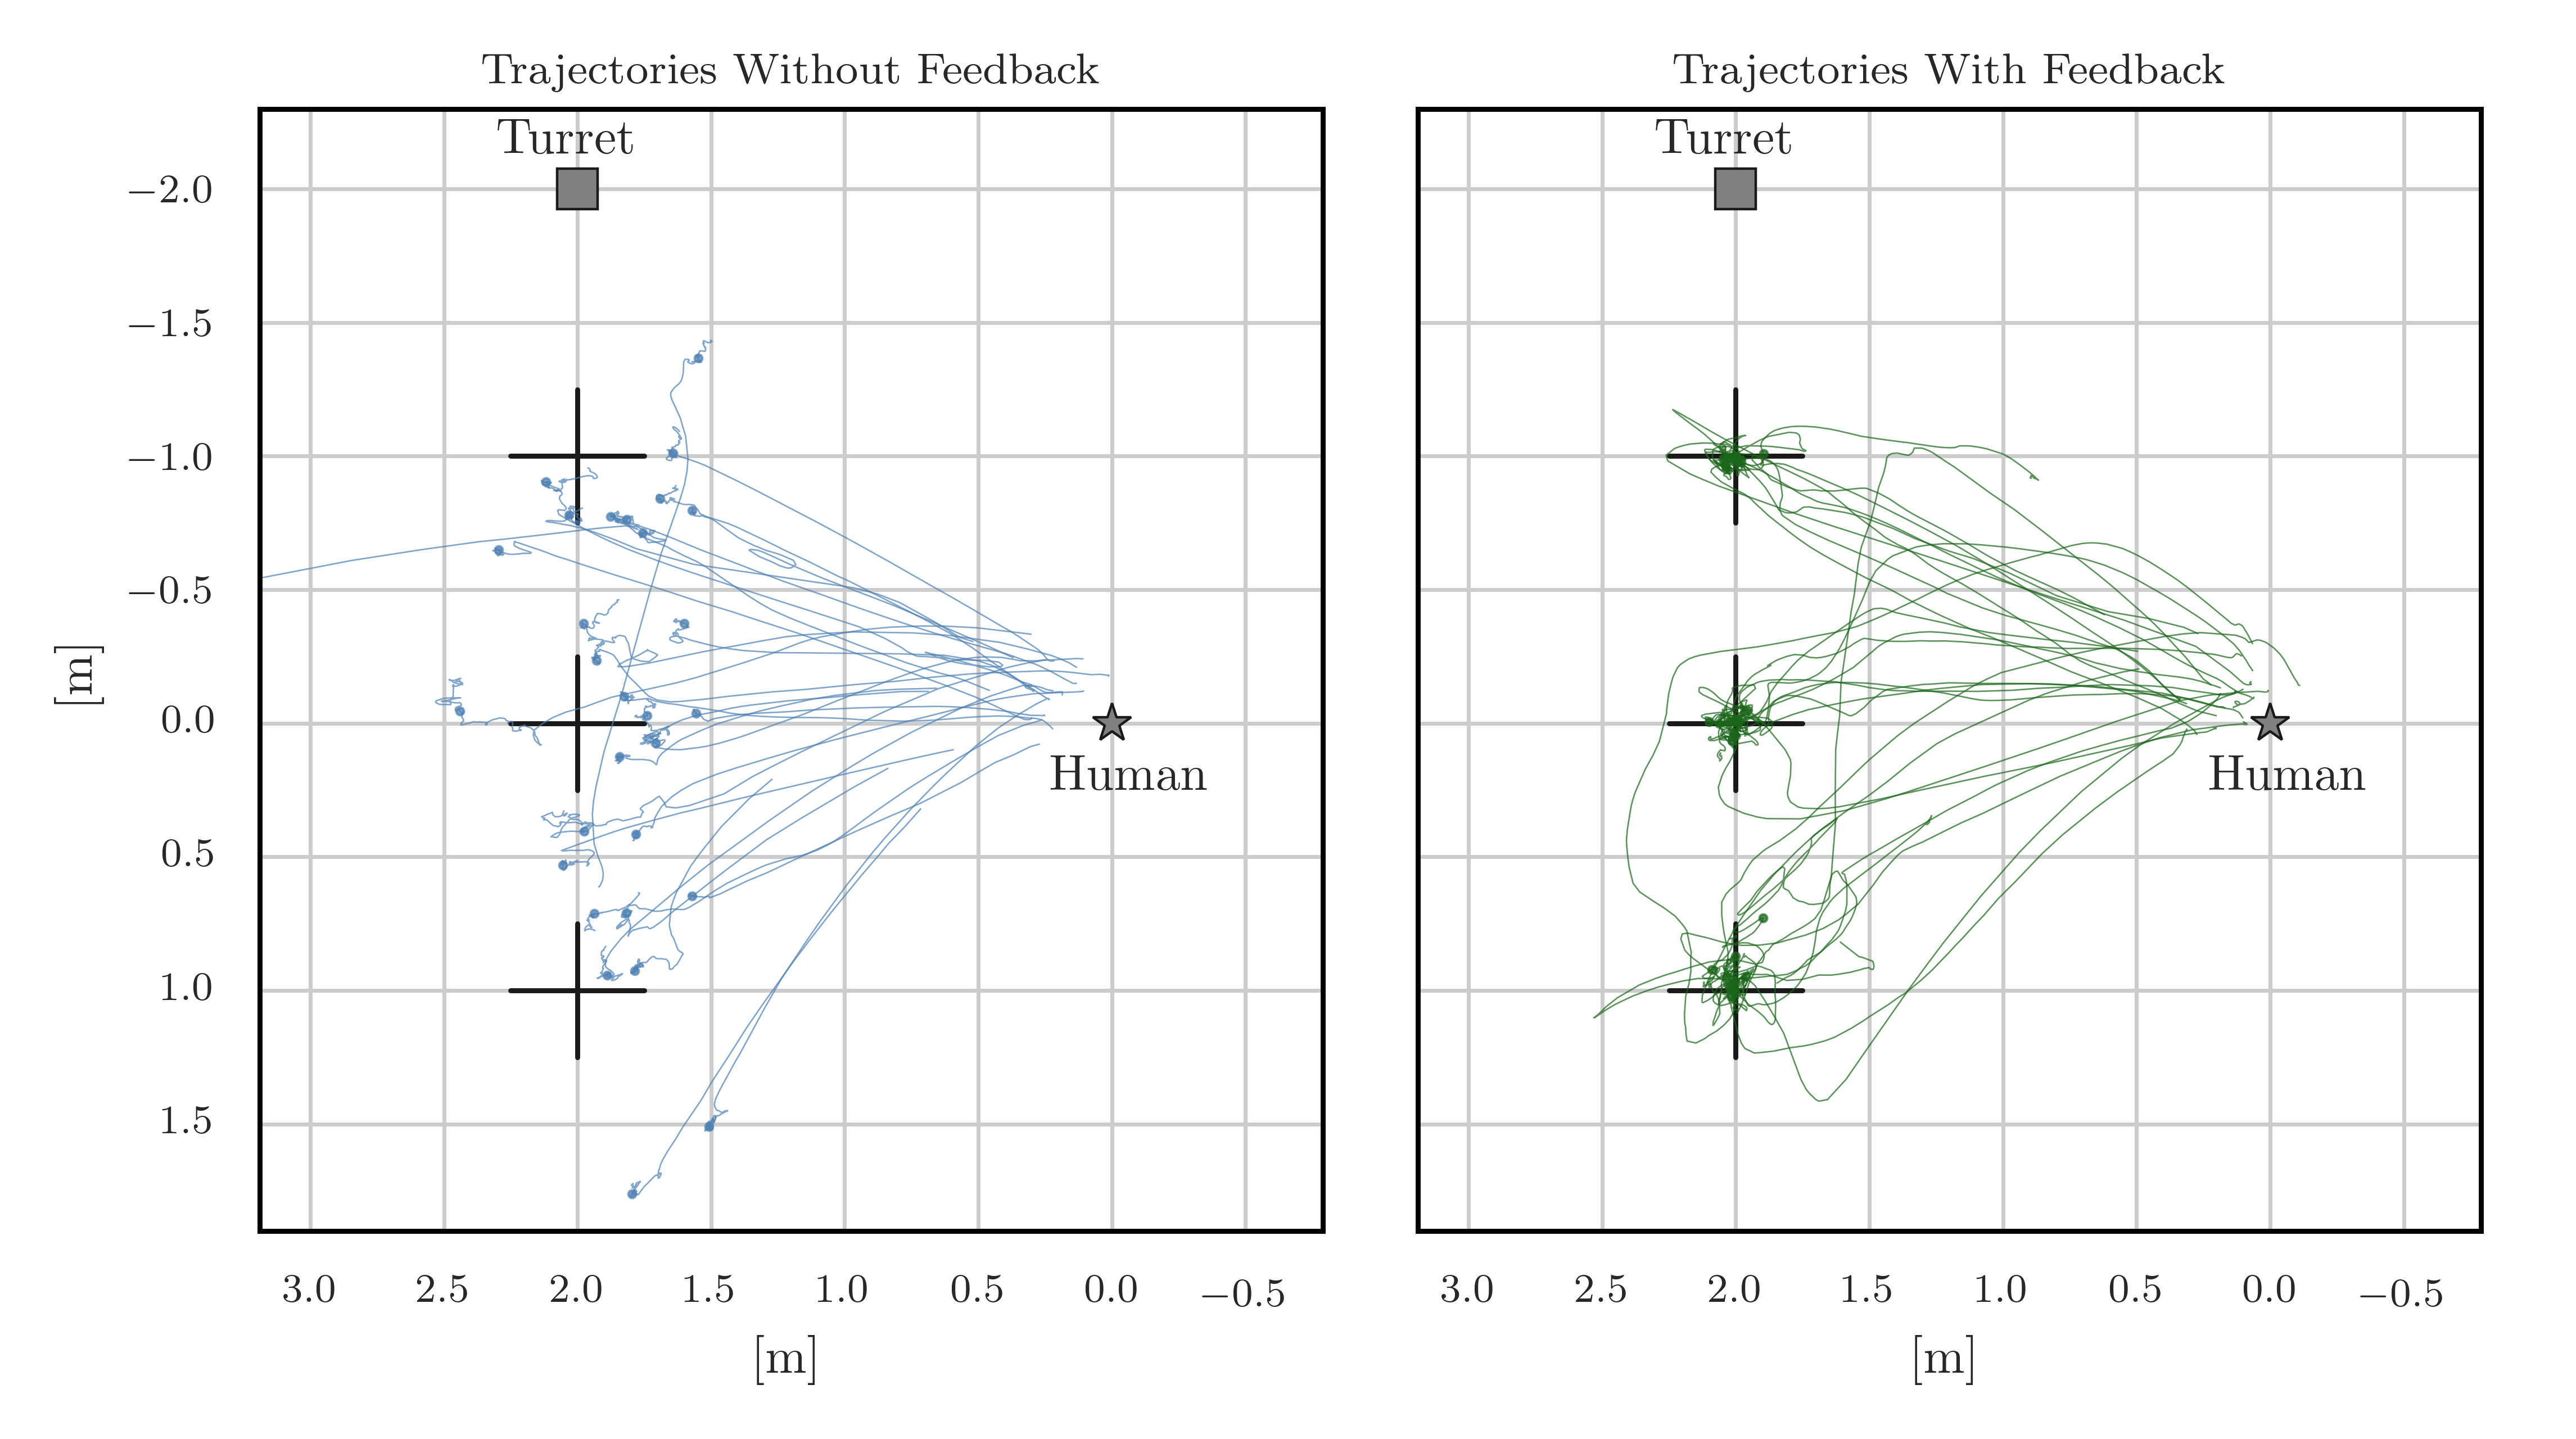
\includegraphics[width=\textwidth]{img/userTrajectories.png}%
	\caption{Users' Trajectories With and Without Feedback}
	\label{fig:userTrajectories}
\end{figure}
\begin{figure}
	\centering
	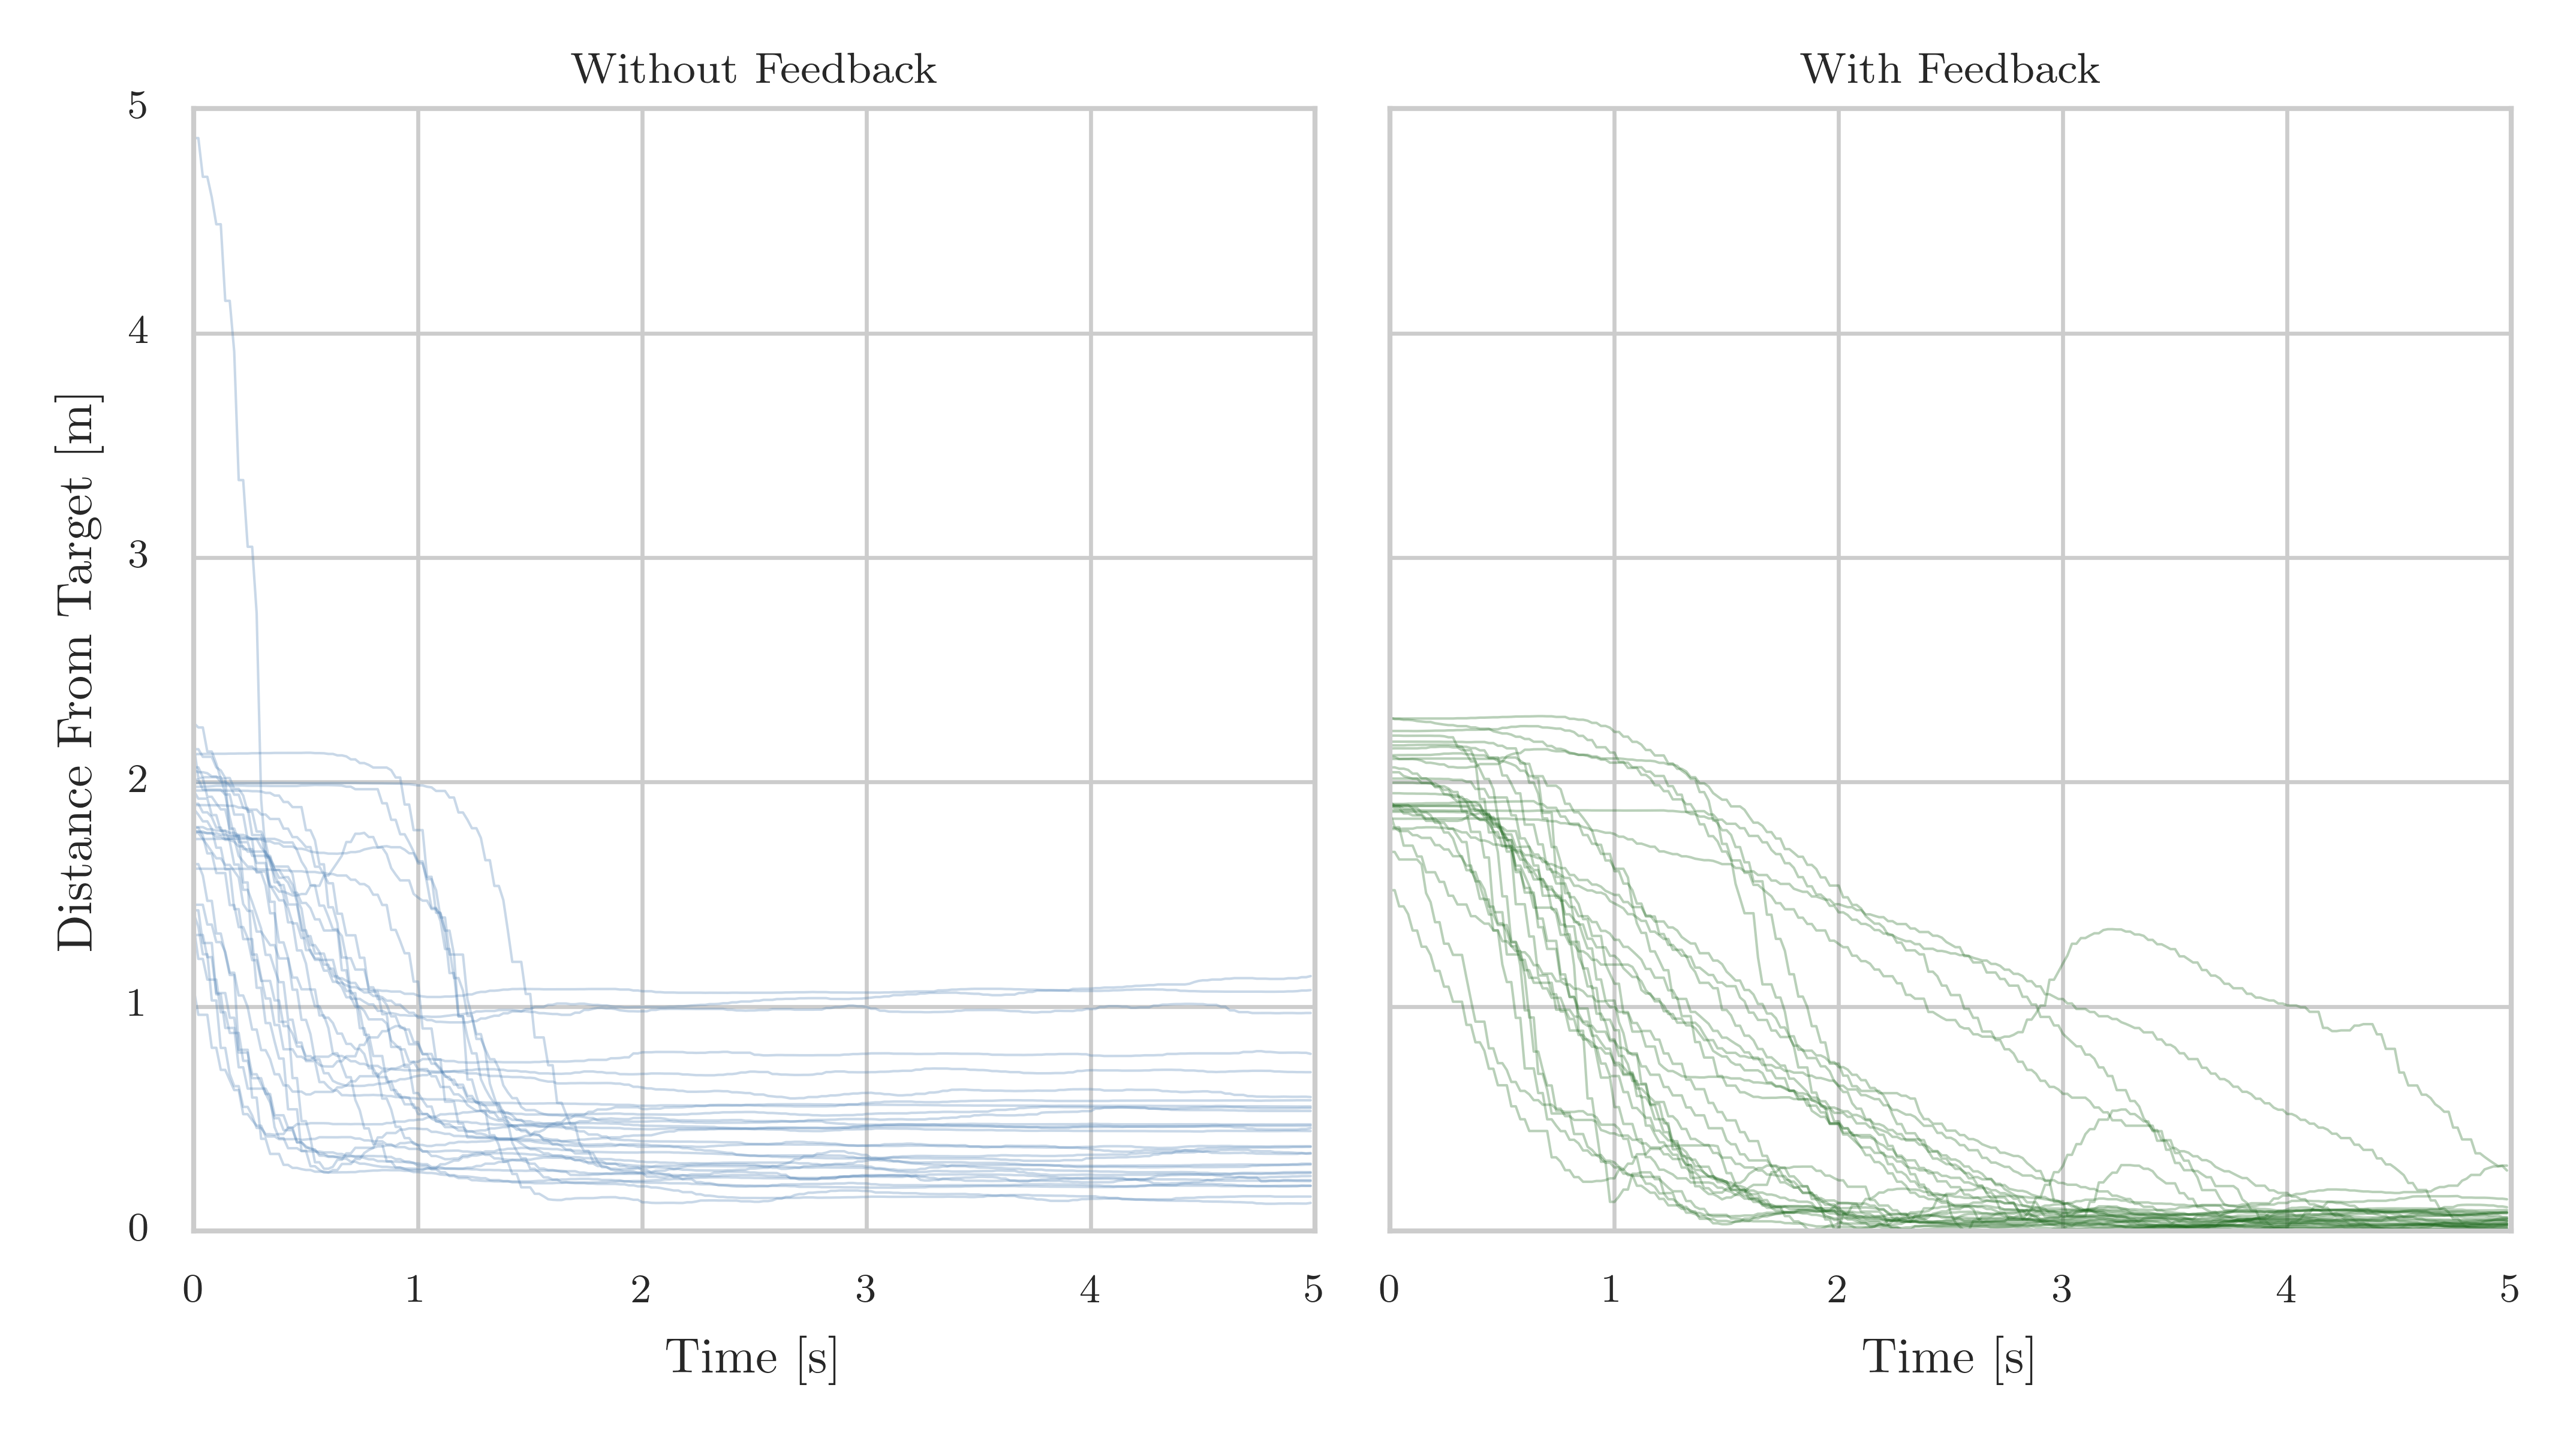
\includegraphics[width=\textwidth]{img/distanceComparison.png}%
	\caption{Comparison Of Distances Over Time}
	\label{fig:distanceComparison}
\end{figure}
\begin{figure}
	\centering
	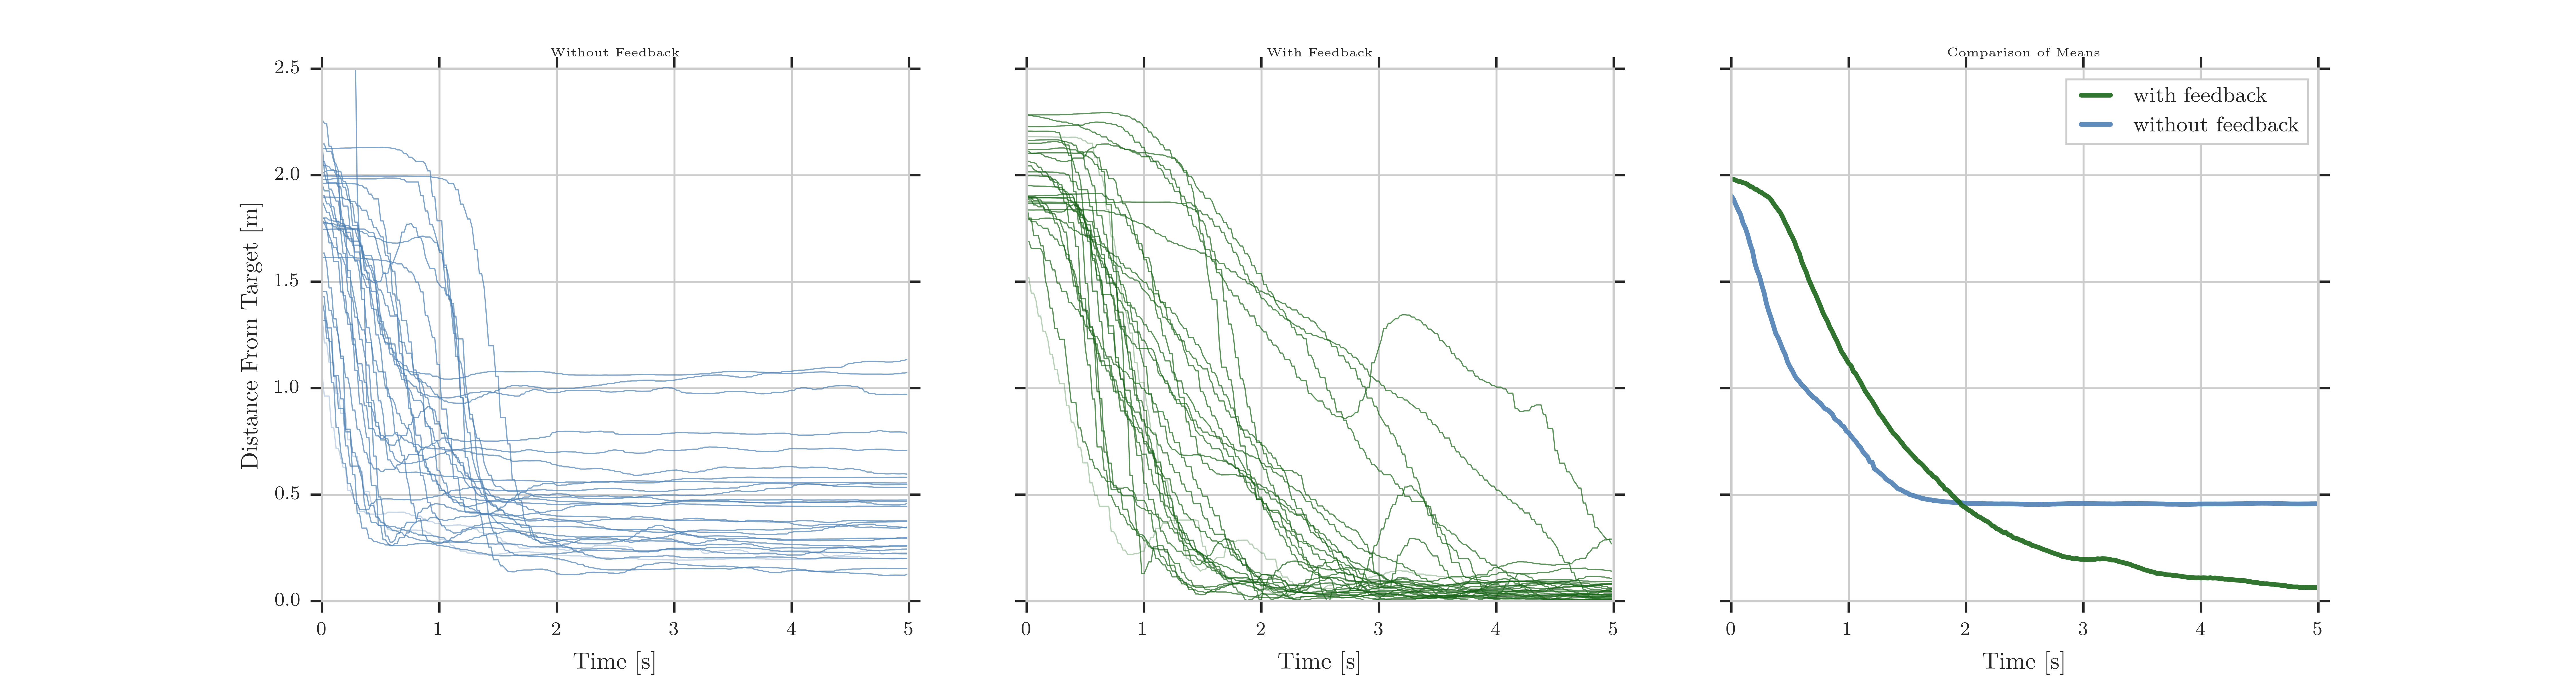
\includegraphics[width=0.7\textwidth]{img/avgDistance.png}%
	\caption{Comparison Of Average Distances Over Time}
	\label{fig:avgDistance}
\end{figure}

\section{Relloc Experiment}
For that experiment we will describe the setup and the goal, but will provide only results obtained with the first turret model, which heavily influenced the results with its limited performance. We have also experimented a bit with the second turret obtaining better qualitative result, but we did not have time to perform an entire data collection with users, which we plan to do in the future.

\subsection{Setup}
We perform the relloc 9 times from 9 different known positions on the floor. The order of the positions is randomly shuffled for each user. So, the experiment runs the following loop 9 time for each user:
\begin{itemize}
    \item the turret points the position where the user must stand and starts a countdown;
    \item at the end of the countdown, the relloc starts: the turret draws the $\infty$ trajectory and the user follow it with pointing gestures;
    \item once the relloc is done, the turret points to the estimated location of the user.
\end{itemize}
In that way we can have an immediate visible the result: the nearer the turret is pointing to the user, the better the relloc is working. We can obtain that measure directly confronting the known initial location with the estimated one.
\begin{figure}
	\centering
	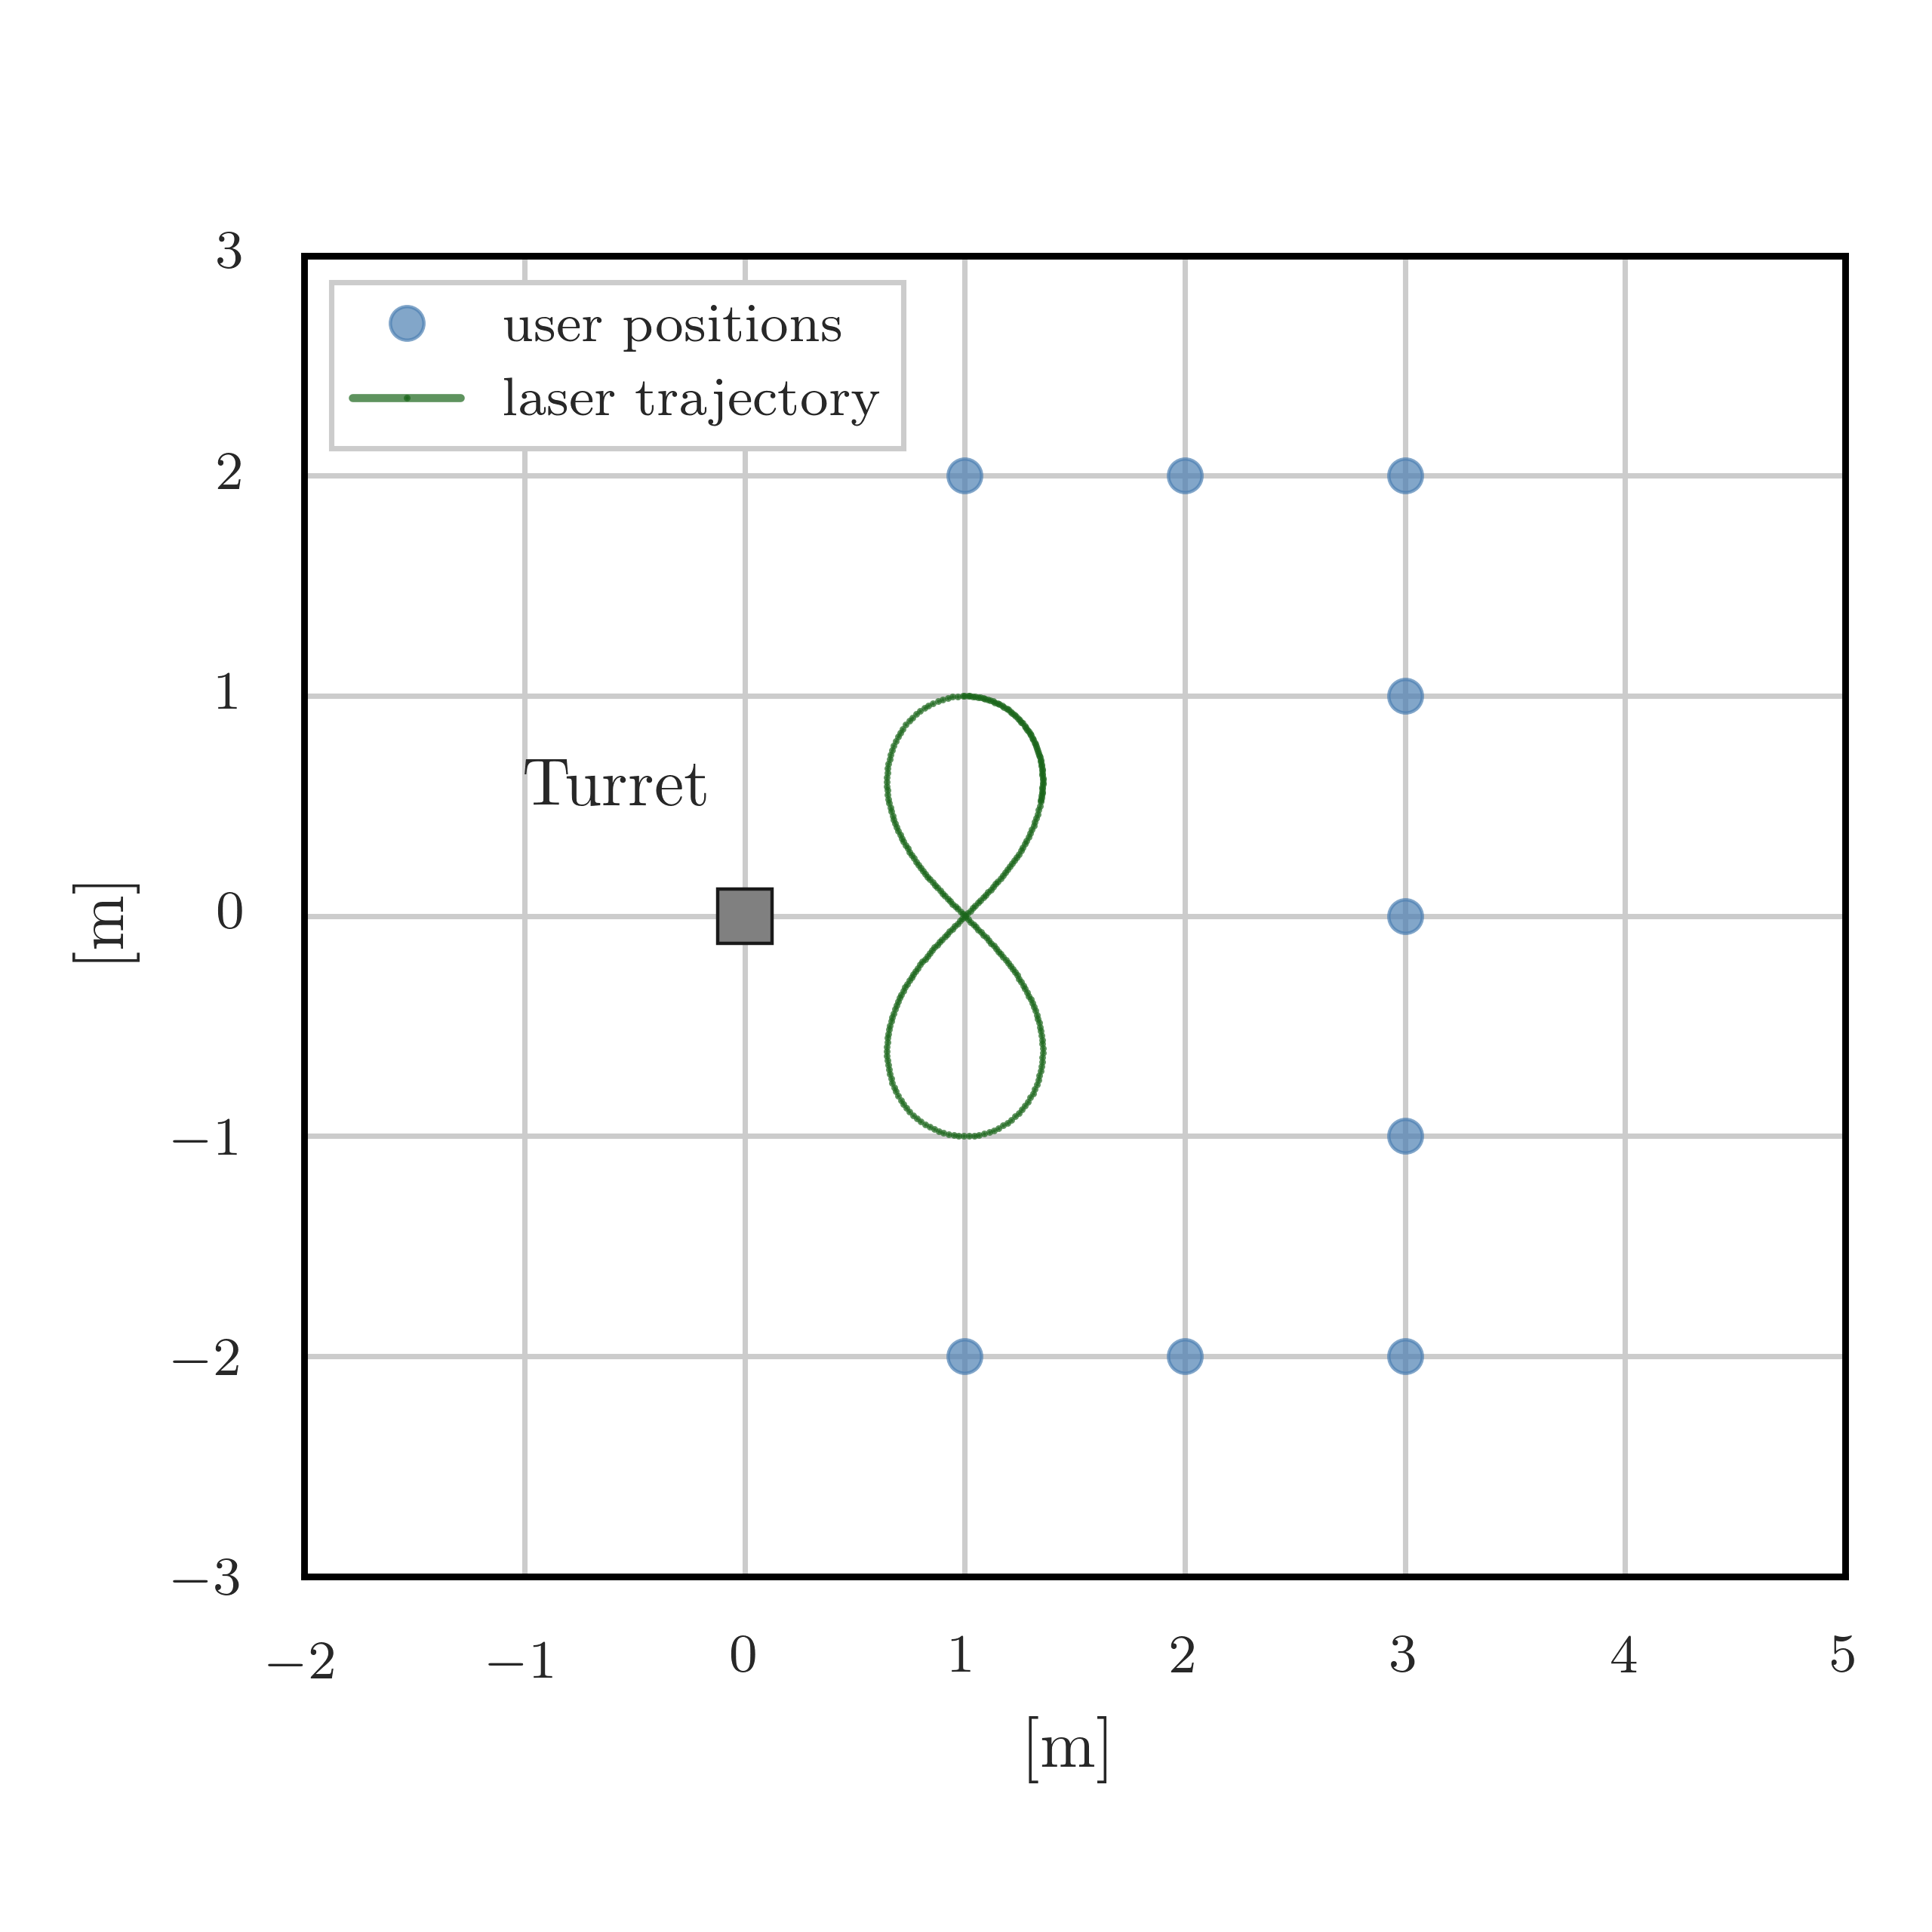
\includegraphics[width=\textwidth]{img/rellocExpSetup.png}%
	\caption{Relloc Experiment Setup}
	\label{fig:pointingExpSetup}
\end{figure}

\subsection{Goals}
The main goals of that experiment of course is to obtain a direct estimate of the relloc precision. Moreover, it is useful to see if also inexperienced users can interface with the system easily.

\subsection{Results}
As already said, we collected data only with the first turret model. We will also run the experiment with the second turret, but from the trials we already did, we have qualitative evidence that the second should obtain better results than the first. \\
However, we report the average error obtained with the data collected with the first turret:
\begin{align}
    \text{mean\_distance\_error} =&\ 48.74\text{ cm} \nonumber\\
    \text{mean\_x\_error} =&\ 36.71\text{ cm}\nonumber\\
    \text{mean\_y\_error} =&\ 24.60\text{ cm}\nonumber
\end{align}
where \textbf{mean\_distance\_error} is the mean of the distances between the position where the user is supposed to be when starting the relloc and the position estimated by our system. \textbf{mean\_x/y\_error} are the means of the differences between each coordinates.

\section{Applications}
As already mentioned, we explored a couple of applications for our system. One consists exactly in what was done for the experiments already presented. In fact, that system is useful to collect data and study pointing models. It also serves as a tool to asses the performances and the precision of the relloc procedure.\\
However, in that section will we present two entire human-robot interaction scenarios involving a ground robot (the kobuki) as well as the turret.\\
A video containing both of them is available at \todo{ref al video}

\subsection{Kobuki Go to Goal Application}
The original relloc system was applied to control a flying robot \cite{gromov2018robot}. In that context, the feedback user had while controlling the drone with pointing consisted of the drone itself. However, that approach is not suitable for a slow moving ground robot, as the kobuki. Here the turret system comes in play: mounting it on top of the kobuki, we can face the mobile robot navigation task in a convenient way.\\
Figure \ref{fig:kgtgSetup} the setup of the demo: we have the user wearing the IMU device and the kobuki equipped with our turret. The steps composing the demo are the following:
\begin{itemize}
    \item the user does the relloc (figure \ref{fig:kgtgRelloc});
    \item an audio feedback alerts the user that the relloc is done and he can now move the laser with pointing;
    \item the user points the place he wants the kobuki to reach for three second (figure \ref{fig:kgtgPointing});
    \item the kobuki moves to that point, while the laser keeps pointing at it. (figure \ref{fig:kgtgGoal})
\end{itemize}
Figure \ref{fig:kgtgGoal} gives also a qualitative feedback: the user is able to drive the kobuki through the cones easily and precisely



\begin{figure}
	\centering
	\includegraphics[width=\textwidth]{img/kgtgSetup.png}%
	\caption{Kobuki Go to Goal Demo: Setup}
	\label{fig:kgtgSetup}
\end{figure}
\begin{figure}
	\centering
	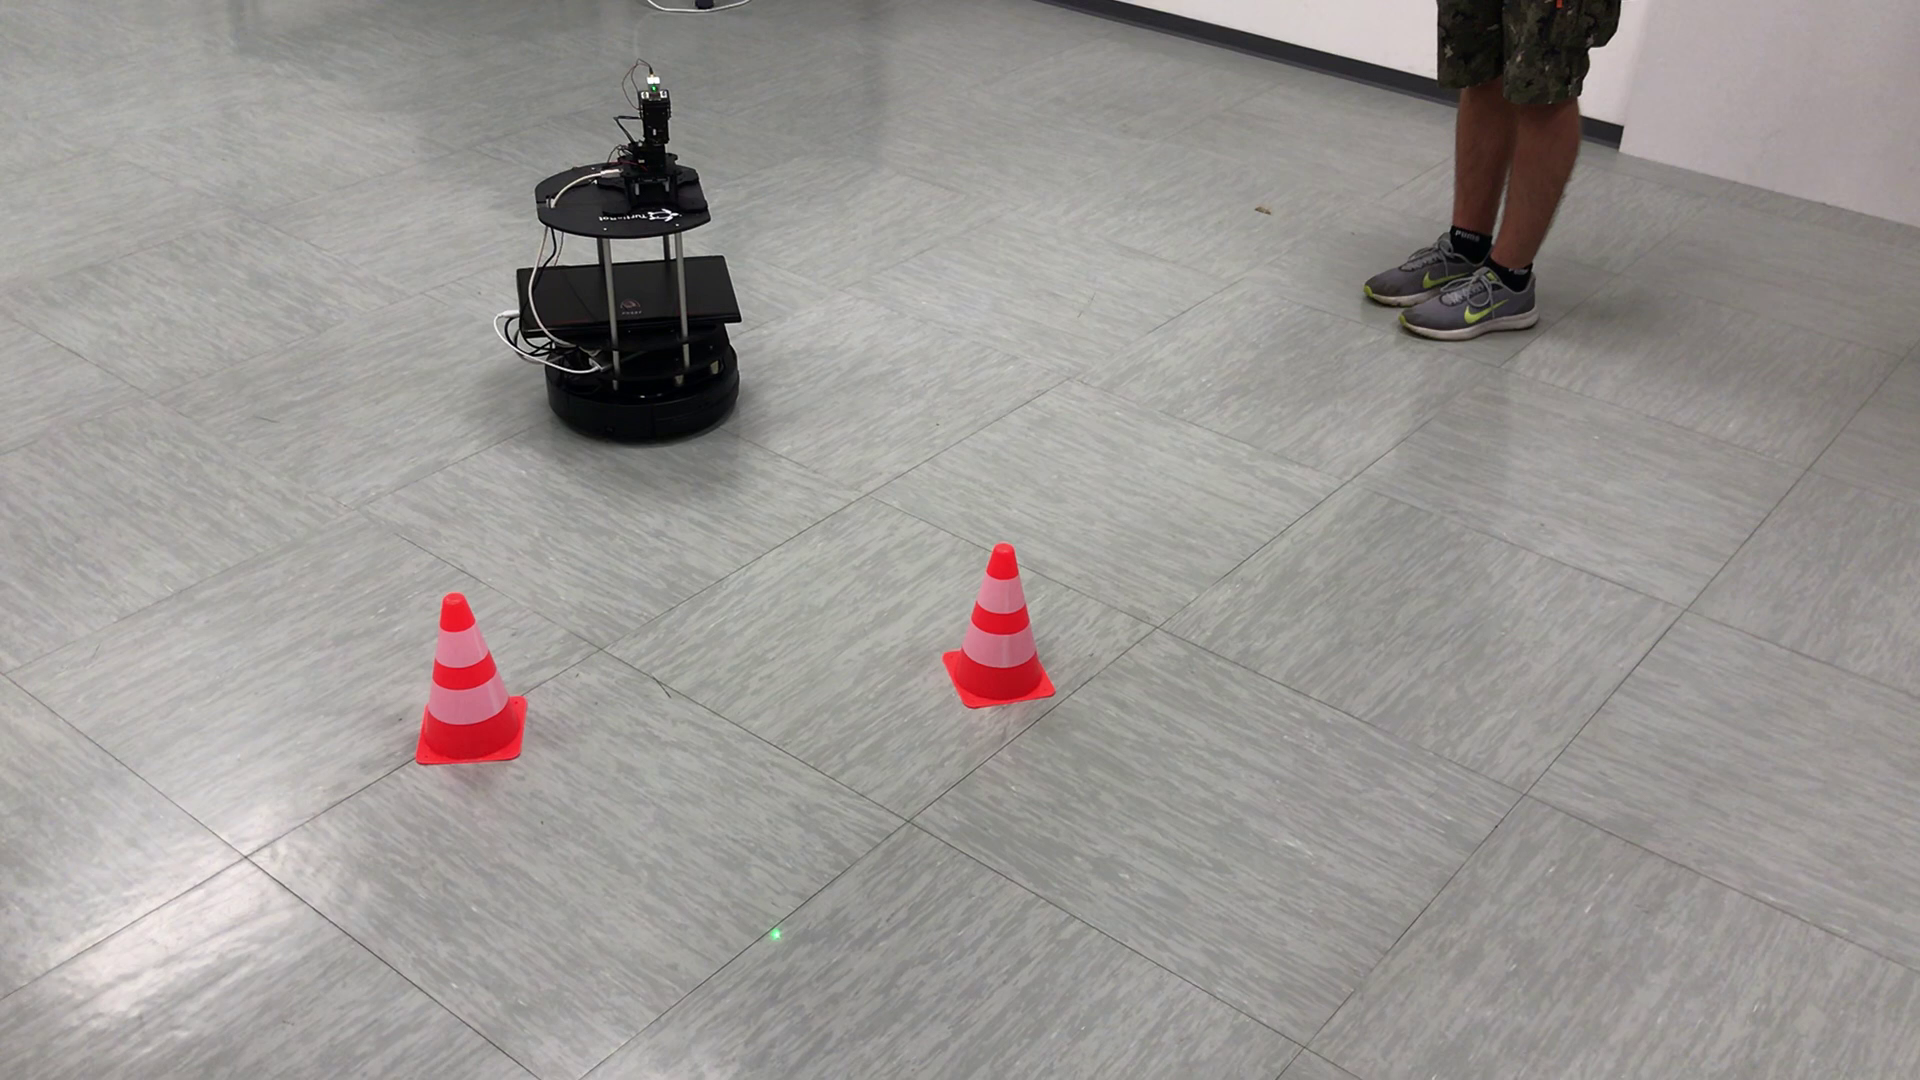
\includegraphics[width=\textwidth]{img/kgtgPointing.png}%
	\caption{Kobuki Go to Goal Demo: Pointing Goal Point}
	\label{fig:kgtgPointing}
\end{figure}

\begin{figure}
	\centering
	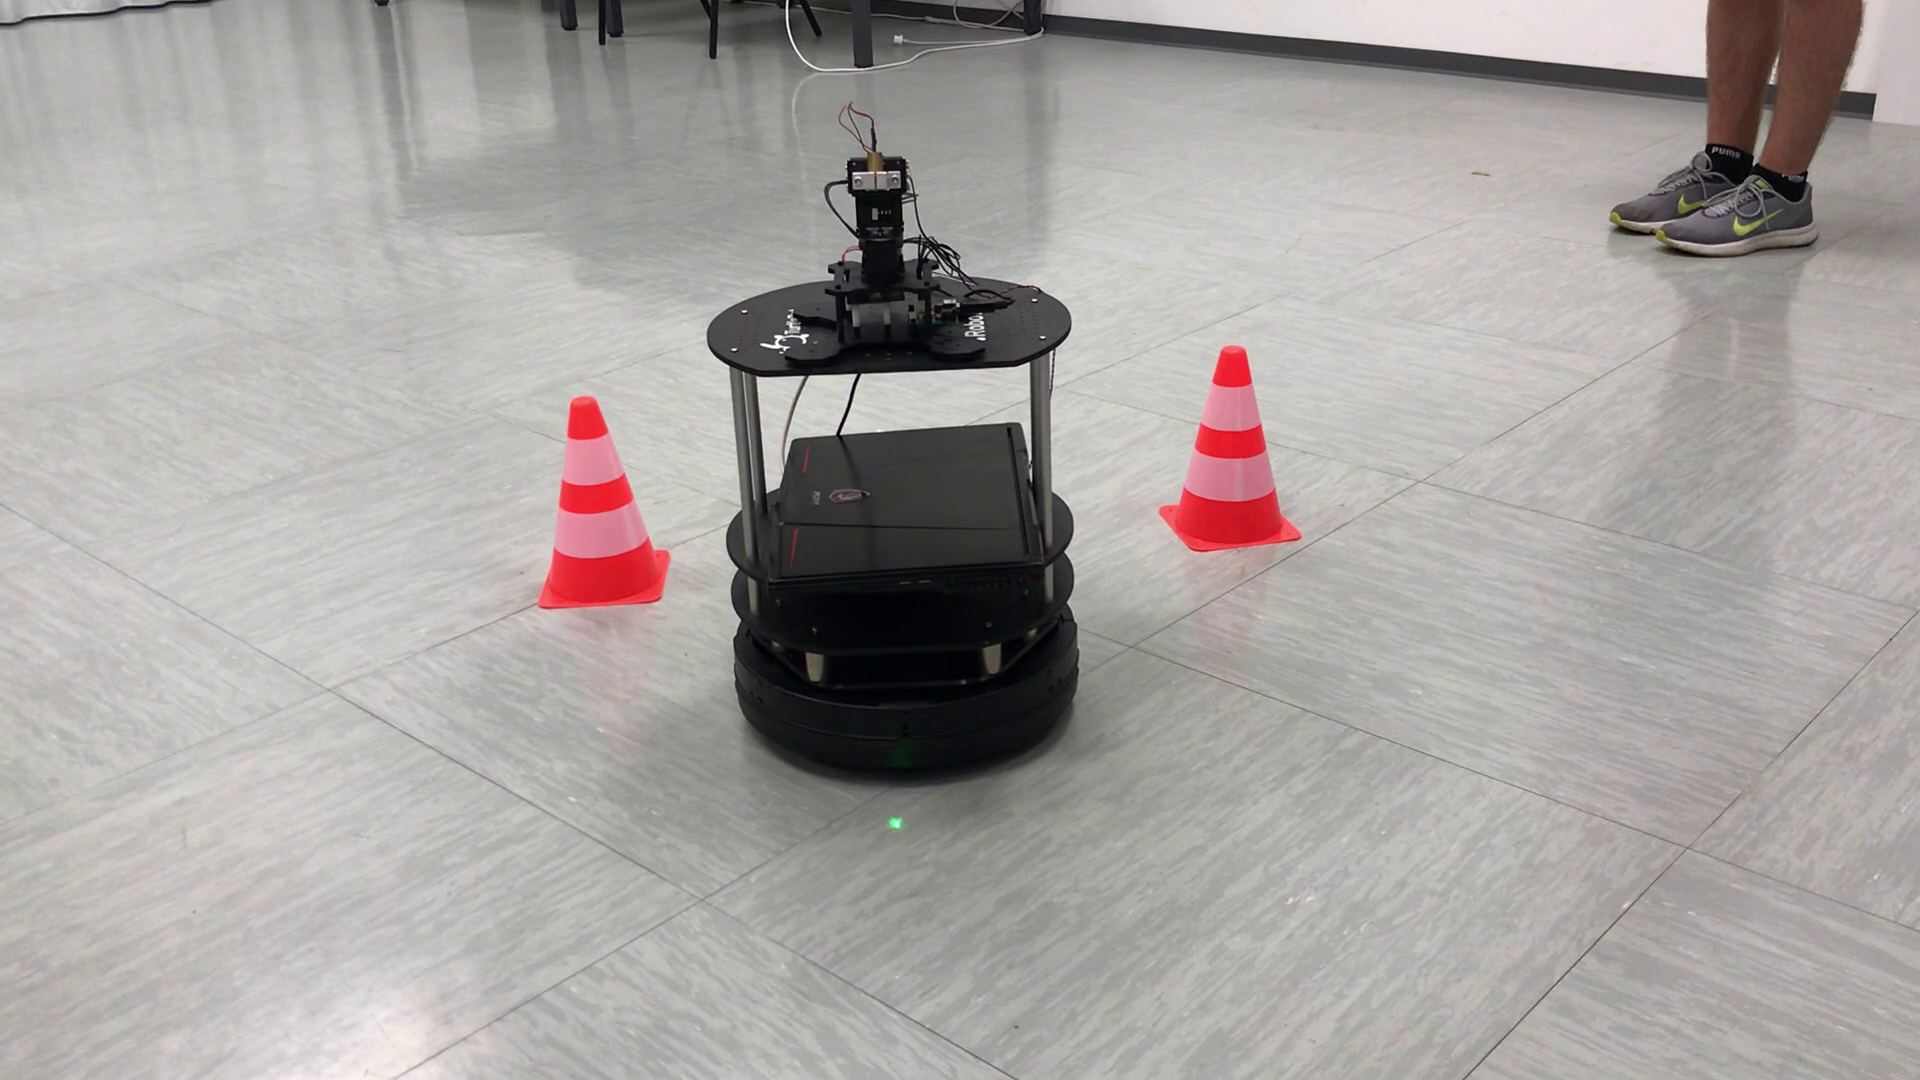
\includegraphics[width=\textwidth]{img/kgtgGoal.png}%
	\caption{Kobuki Go to Goal Demo: Goal Point Reached}
	\label{fig:kgtgGoal}
\end{figure}